\documentclass{article}
\usepackage{tikz}
\usetikzlibrary{arrows.meta,positioning,calc,shapes.geometric}
\pagestyle{empty}
\begin{document}
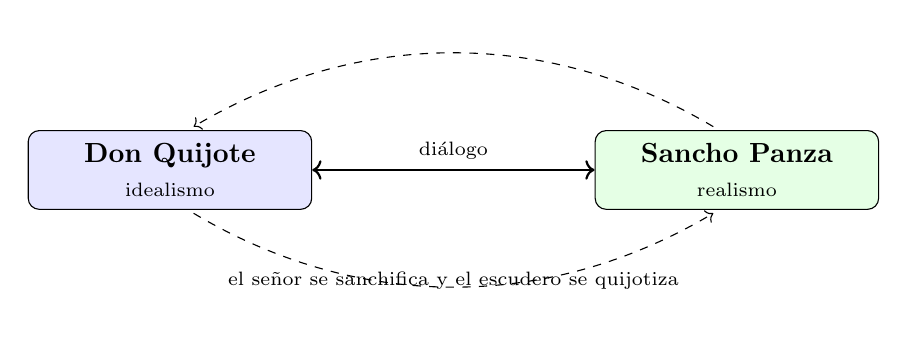
\begin{tikzpicture}
\tikzset{every node/.append style={align=center}}

\node[draw, rounded corners, fill=blue!10, minimum width=3.6cm, minimum height=1.0cm, align=center] (q) at (0,0) {\textbf{Don Quijote}\\ \scriptsize idealismo};
\node[draw, rounded corners, fill=green!10, minimum width=3.6cm, minimum height=1.0cm, align=center] (s) at (7.2,0) {\textbf{Sancho Panza}\\ \scriptsize realismo};
\draw[<->, thick] (q) -- node[above, font=\scriptsize] {diálogo} (s);
\node[font=\scriptsize, align=center] at (3.6,-1.4) {el señor se sanchifica y el escudero se quijotiza};
\draw[->, dashed] (0.3,-0.55) .. controls (2.4,-1.8) and (4.8,-1.8) .. (6.9,-0.55);
\draw[->, dashed] (6.9,0.55) .. controls (4.8,1.8) and (2.4,1.8) .. (0.3,0.55);

\end{tikzpicture}
\end{document}
